	\documentclass{lebook}

	% This document requires the use of Lance A. Endres's LaTeX library available at the following location:
	% https://github.com/lendres/LaTeX

%%%%%%%%%%%%%%%%%%%%%%%%%%%%%%%%%%%%%%%%%%%%%%%%%%%%%%%%%%%%%%%%%%%%%%%%%%%%%%%%%%%%%%%%%%%%
% Notes to do:
% - Convert the figure "" in impurity section to a table.
% - Create a table of Accuracy, Recall, Precision, and F1 comparisons.
%%%%%%%%%%%%%%%%%%%%%%%%%%%%%%%%%%%%%%%%%%%%%%%%%%%%%%%%%%%%%%%%%%%%%%%%%%%%%%%%%%%%%%%%%%%%

%%%%%%%%%%%%%%%%%%%%%%%%%%%%%%%%%%%%%%%%%%%%%%%%%%%%%%%%%%%%%%%%%%%%%%%%%%%%%%%%%%%%%%%%%%%%
% Code to do:
%%%%%%%%%%%%%%%%%%%%%%%%%%%%%%%%%%%%%%%%%%%%%%%%%%%%%%%%%%%%%%%%%%%%%%%%%%%%%%%%%%%%%%%%%%%%

	% SETUP
	\input{"Setup.tex"}

	\begin{document}

	\input{"Equations.tex"}

    % MAKE A TITLE PAGE.
	\input{"Title Page.tex"}

	\pagestyle{leplainheader}
	\frontmatter{}

	% GENERATE THE TABLE OF CONTENTS.
	\tableofcontents{}
	\listoffigures{}
	\listoftables{}

	\mainmatter{}


	\begin{bulletedlist}
		\item
		\begin{bulletedlist}
			\item
		\end{bulletedlist}
	\end{bulletedlist}

	\begin{figure}[tbh]
		\centering
		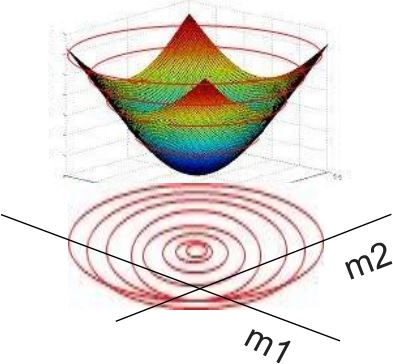
\includegraphics[width=2.0in]{ridgeversuslasso1}
		\caption[]{}
		\label{fig:ridgeversuslasso1}
	\end{figure} 


	% Glossary entries need to be defined before they can be referenced.
	\input{"Statistics Glossary"}
	\input{"Modeling Glossary"}
	\input{"Acronyms"}

	\input{"Statistics"}
	\input{"Data Analysis"}

	\input{"Modeling"}

	\input{"Regression"}
	\input{"Ensemble Techniques"}
	\input{"Feature Selection, Model Selection, and Tuning"}
	\input{"Machine Learning Pipeline and Hyperparameter Tuning"}
	\input{"Clustering"}
	\input{"K-means Clustering"}
	\input{"Hierarchical Clustering and PCA"}

	\input{"Deep Learning Prework"}
	\input{"Introduction to Deep Neural Networks"}
	\input{"Building Blocks of Neural Networks"}
	\input{"Neural Network Troubleshooting"}
	\input{"Computer Vision Prework"}
	\input{"Convolutional Neural Networks"}

	\appendix
	\input{"Interview Questions"}
	\input{"Installation Notes"}

	\backmatter{}
	\pagestyle{leplainheader}



%	% Standard glossary entries.
%	\newglossaryentry{utc}{name=UTC, description={Coordinated Universal Time}}
%	%\gls{utc}
%	\printglossary[type=main, title=General Glossary]{}
%	\renewcommand*{\chaptertitle}{General Glossary}

	% Statistics glossary.
	\printglossary[type=stats, title=Statistics Glossary]{}
	\renewcommand*{\chaptertitle}{Statistics Glossary}

	% Modeling glossary.
	\printglossary[type=model, title=Modeling Glossary]{}
	\renewcommand*{\chaptertitle}{Modeling Glossary}

	% Acronyms.
	\printglossary[type=\acronymtype]
	\renewcommand*{\chaptertitle}{Acronyms}

	% PRINT A LIST OF NOTATIONS / NOMENCLATURE.
	% Argument is a text/tex file containing lines in the form of:
	% \addnotation{Variable}{Meaning of variable.}
	\input{"List of Notations.tex"}

	% Use all glossary entries without specifically referencing them.
	% Gather all unused glossary terms.  Putting it before "\printgossaries" seems to cause a blank page to be injected.
	\glsaddallunused{}

	\bibliography{le,machinelearning}

	\end{document}
